\section{\iflanguage{english}{Kissat Results}{Kissat Ergebnisse}}\label{sec:kissat_results}

In diesem Kapitel werden die experimentellen Ergebnisse zur Bewertung der Auswirkungen der 
Algorithmusauswahl und der Vorverarbeitung durch SATZilla auf verschiedene Varianten des Kissat-Lösers 
vorgestellt.

Die Idee hier ist zu testen was Passiert wenn man Satzilla, wieder Trainiert auf unseren Kissat variationen, 
nicht auf die ursprünglichen Benchamrks sondern auf die gleichen Benchmarks in vereinfachter form.

In realen SAT-Lösungsabläufen wird vor der Lösung üblicherweise eine Vorverarbeitung durchgeführt. 
Vorverarbeitungstechniken wie Variableneliminierung, Subsumption und Äquivalenzschluss vereinfachen 
die Formel, indem sie redundante Klauseln und Variablen entfernen. Die Vorverarbeitung kann zwar 
den Umfang der Formel und die Lösungszeit drastisch reduzieren, verändert jedoch auch die 
strukturellen Eigenschaften der Formel, auf deren Erfassung die Funktionen von SATZilla ausgelegt sind.

Die Forschungslücke: Der ursprüngliche Featuresextraktor und Algorithmusauswähler von SATZilla wurden 
anhand von ursprünglichen, unverarbeiteten Benchmarks entwickelt und evaluiert. Es ist nicht bekannt, ob 
die Vorhersagen von SATZilla auch dann gültig bleiben, wenn sie auf vorverarbeitete Formeln angewendet 
werden. Dies führt zu einem praktischen Problem:

\textit{Wenn ein Benutzer seine SAT-Instanz vor dem Ausführen eines Solvers vorverarbeitet, kann er dann 
dennoch der Solver-Empfehlung von SATZilla vertrauen, oder macht die Vorverarbeitung die Merkmale 
und damit die Vorhersage ungültig?}

Hierführ bekam ich von meinem Tutor zwei neue Dateien mit den Namen: \textbf{sc2024pre10k} und 
\textbf{sc2024pre100k}, wobei 10k \& 100k jeweils für eine Vereinfachung von 10.000 und 100.000 fur die 
Benchmarks stehen.

Die Idee ist nun mit dem trainierten Satzilla model zu vergleichen wie sich die Predicitons unterscheiden
mit dem ursprünlgichen und vereinfachten Benchmarks und was wir daraus schließen können.

Zum Schluss werde ich untersuchen ob die Laufzeiten von den vereinfachten Benmchamrks verglichen mit dem 


\subsection{Setup}

\textbf{Training Data:}
\begin{itemize}
    \item 400 SAT benchmarks aus der SAT Wettbewerb
    \item 6 Kissat Solver varianten:
\end{itemize}

\begin{quote}
    \textbf{kissat\_default} \\
    \textbf{kissat\_noeliminate} \\
    \textbf{kissat\_nostable} \\
    \textbf{kissat\_stable} \\
    \textbf{kissat\_stable2} \\
    \textbf{kissat\_target2} 
\end{quote}

\begin{itemize}
    \item Laufzeit Data aus kissat-strategy-runs.tar.xz
\end{itemize}

\textbf{Test Data}
\begin{itemize}
    \item 324 gemeinsame Instanzen der drei Versionen:
\end{itemize}

\begin{quote}
    \textbf{Original}: Unbearbeitete Benchmarks \\
    \textbf{Pre10k}: Leicht vereinfachte Benchamrks (10.000 Vorverarbeitungsschritte) \\
    \textbf{Pre100k}: stark vereinfachte Benchmarks (100.000 Vorverarbeitungsschritte)
\end{quote}

\subsubsection{Feature Extraction Process}

Der Grund für die 324 gemeinsamen Instanzen liegt am Featuresextraktor.

Die Features  wurden mit dem SATZilla 2024-Featurextraktor extrahiert, wobei pro Merkmalsgruppe ein 
Zeitlimit von 180 Sekunden galt. Der Featuresextraktor Prozess umfasste:

\verb|./features -all -t 180 <benchmark.cnf> <output_features.csv>|

\newpage

\begin{table}[H]
    \centering
    \begin{tabular}{lccc}
        \textbf{Dataset} & \textbf{Benchmarks} & \textbf{Erfolgreiche Extraktionen} \\
        \toprule
        Original & 400 & 400 \\
        \midrule
        Pre10k & 348 & 348 \\
        \midrule
        Pre100k & 324 & 324  \\
        \bottomrule
    \end{tabular}
    \caption{Feature Extraction Statistics}\label{tab:extraction_stats}
\end{table}

Während der Vorverarbeitung (Vereinfachung) wurden einige Testfälle bereits vollständig gelöst 
(SAT/UNSAT ermittelt), noch bevor der Solver überhaupt gestartet war.

Durch stärkere Vereinfachung wurden auch mehr Benchmarks gelöst, so wurden von Pre10k 52 der benchmarks 
beretis gelöst und 76 Benchamrks von Pre100k.

Somit haben wir letztendlich 324 gemeinsame Benchmarks zum vergleichen.

\newpage

\subsubsection{SATZilla Model Training}

Das Model wurde wieder wie in Kapitel 3 Beschrieben trainiert.

Ein Random-Forest-Klassifikator wurde mit den folgenden Hyperparametern trainiert:

\begin{table}[H]
    \centering
    \begin{tabular}{ll}
        \toprule
        \textbf{Parameter} & \textbf{Wert} \\
        \midrule
        Anzahl der Bäume & 200 \\
        \midrule
        Maximale Tiefe & 20 \\
        \midrule
        Minimale Samples für Split & 5 \\
        \midrule
        Klassen-Gewichtung & Ausgeglichen (Balanced) \\
        \midrule
        Zufallsstartwert (Random state) & 42 \\
        \midrule
        Train/Test Aufteilung & 80/20 (stratifiziert) \\
        \bottomrule
    \end{tabular}
    \caption{Random Forest Konfigurationsparameter}\label{tab:rf_params}
\end{table}

\textbf{Trainingsergebnisse}

Die Trainingsergebnisse waren mit einer Testgenauigkeit von 43.08 \% wider sehr Ähnlich unserem Ergebnissen
aus Kapitel 3 und somit zuferlässig genug um jetzt verhersagen auf unseren Verinfachten Benchmarks durchzuführen.

\newpage

\subsection{Auswirkungen der Vorverarbeitung auf die Vorhersagen von SATZilla}

\textbf{Forschungsfrage}

Beeinflusst die Vorverarbeitung (Vereinfachung) von SAT-Instanzen die Vorhersagen von SATZilla zur 
Solverauswahl?

Meine Vermutung liegt darin das sich die Vorhersagen der Solver bestimmt ändern muss, da SATZilla die 
Sover demenentsprechend der Features auswählt, ändern sich somit die Features sollte sich doch 
ebenfalls die Vorhersage des Solvers in einigen Fällen ändern.

Wie groß diese Ändereungen sein werden und ob eine stärkere Verinfachung zu noch größeren Veränderungen 
der Solver Auswahl haben wird werden wir jetzt sehen.

\subsubsection{Veränderungen der Vorhersageverteilung}

Jetzt die Grafik meiner Ergebnisse die darstellt wie sich die Solver Verteilung der drei 
verschiedenen benchmarks darstellt.

\begin{figure}[H]
    \centering
    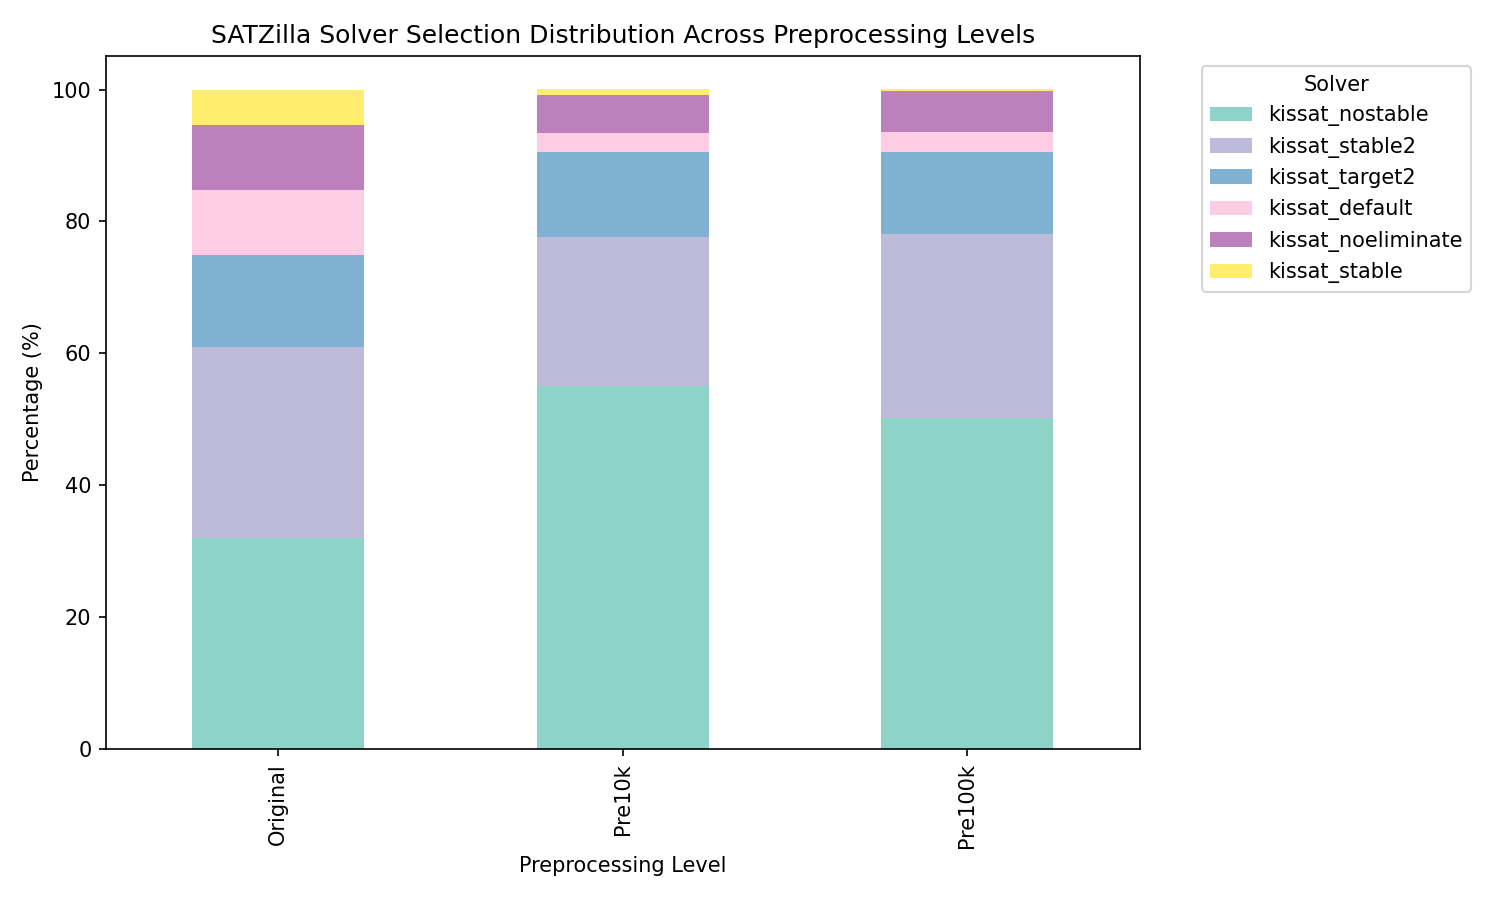
\includegraphics[width=0.8\textwidth]{assets/solver_distribution.png}
    \caption{Solver-Verteilung für Original-, Pre10k- und Pre100k-Benchmarks}
    \label{fig:solver_distribution}
\end{figure}

Die Grafik zeigt, wie sich die Solver-Empfehlungen von SATZilla bei denselben 324 Benchmarks je nach 
Vorverarbeitungsstufe unterscheiden.

Meine Vermutung lag richtig und man kann erkennen das sich die Solver Empfehlung verändert hat aber 
so das man immer noch eine gewisse ähnlichkeit erkennen kann vor jeder Vereinfachung.

Die Verschiebung der Verteilung zeigt, dass die Vorverarbeitung nicht alle Solver gleichermaßen 
beeinflusst. kissat\_nostable erwies sich nach der Vorverarbeitung als die vorherrschende 
Empfehlung (50,2 \%), während kissat\_stable fast nie empfohlen wurde (0,3 \%). Dies deutet darauf hin, 
dass die Heuristik der stabilen Phase, die bei ursprünglichen Formeln von Vorteil ist, ihren Vorteil 
bei vereinfachten Formeln verliert. Umgekehrt scheint die nostable-Konfiguration, die die stabile 
Phase deaktiviert, für vorverarbeitete Instanzen besonders gut geeignet zu sein.

\textbf{Verteilung der Solver-Auswahl (\%)}

\begin{table}[H]
    \centering
    \begin{tabular}{lccc}
        \toprule
        \textbf{Solver} & \textbf{Original} & \textbf{Pre10k} & \textbf{Pre100k} \\
        \midrule
        kissat\_nostable & 31.9\% & 55.1\% & 50.2\% \\
        \midrule
        kissat\_stable2 & 29.1\% & 22.6\% & 27.9\% \\
        \midrule
        kissat\_target2 & 13.9\% & 12.8\% & 12.4\% \\
        \midrule
        kissat\_default & 9.9\% & 2.9\% & 3.1\% \\
        \midrule
        kissat\_noeliminate & 9.9\% & 5.8\% & 6.2\% \\
        \midrule
        kissat\_stable & 5.3\% & 0.9\% & 0.3\% \\
        \bottomrule
    \end{tabular}
    \caption{Solver Selection Distribution (\%)}\label{tab:solver_distribution}
\end{table}

\subsubsection{Änderungen der Vorhersagen nach Vorverarbeitungsstufe}

Hier die Anzahl an veränderten Instanzen im Vergleich von \textbf{Original}, \textbf{Pre10k} und \textbf{Pre100k}

\begin{figure}[H]
    \centering
    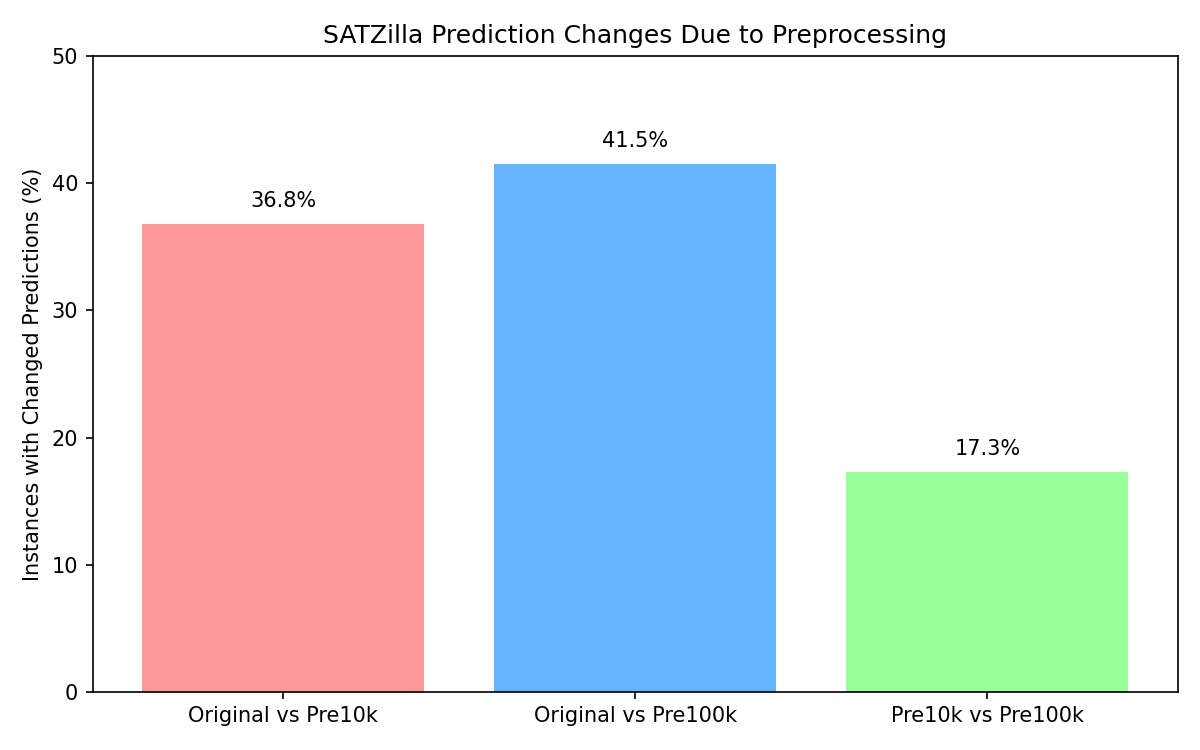
\includegraphics[width=0.8\textwidth]{assets/prediction_changes.png}
    \caption{Anzahl der Solver Änderungen für Original-, Pre10k- und Pre100k-Benchmarks}
    \label{fig:prediction_changes}
\end{figure}

Das Balkendiagramm zeigt, dass 36,8 \% der Benchmarks ihre Vorhersagen nach einer leichten 
Vorverarbeitung (Pre10k) geändert haben, wobei dieser Anteil nach einer umfassenden Vorverarbeitung 
(Pre100k) auf 41,5 \% anstieg. Die zusätzliche Veränderung zwischen Pre10k und Pre100k beträgt 
lediglich 17,3 \%, was darauf hindeutet, dass der Großteil der Abweichungen bereits während der 
anfänglichen Vereinfachung auftritt.

\begin{table}[H]
    \centering
    \begin{tabular}{lcc}
        \toprule
        \textbf{Vergleich} & \textbf{Geänderte Instanzen} & \textbf{Prozentsatz} \\
        \midrule
        Original $\rightarrow$ Pre10k & 119 von 323 & 36,8\% \\
        \midrule
        Original $\rightarrow$ Pre100k & 134 von 323 & 41,5\% \\
        \midrule
        Pre10k $\rightarrow$ Pre100k & 56 von 323 & 17,3\% \\
        \bottomrule
    \end{tabular}
    \caption{Vorhersageänderungen zwischen verschiedenen Vorverarbeitungsstufen}\label{tab:prediction_changes}
\end{table}

Wie man sieht änder sich die Solver Empfehlung von \textbf{Original} verglichen mit \textbf{Pre10k} und 
\textbf{Pre100k} um 36.8-41.5\%.

Das bedeutet, dass in mehr als einem Drittel aller Fälle die Vorverarbeitung die Empfehlung 
beispielsweise von „use kissat\_stable2“ in „use kissat\_nostable“ geändert hat.

\newpage

Die meisten Änderungen treten zwischen der Originalversion und der vorverarbeiteten Version auf

Beachte:
\begin{itemize}
    \setlength{\itemsep}{0pt}
    \setlength{\parskip}{0pt}
    \setlength{\parsep}{0pt}
    \item Original $\rightarrow$ Pre10k: 119 Änderungen
    \item Pre10k $\rightarrow$ Pre100k: 56 Änderungen
    \item Original $\rightarrow$ Pre100k: 134 Änderungen
\end{itemize}

Interessante Beobachtung: $119 + 56 = 175$, was größer ist als $134$. Das bedeutet:
\begin{itemize}
    \item Einige Benchmarks änderten sich von Original $\rightarrow$ Pre10k, dann erneut (oder zurück) von Pre10k $\rightarrow$ Pre100k
    \item Andere Benchmarks änderten sich nur zwischen Original und Pre100k (überspringen Pre10k)
\end{itemize}

durch diese Beaobachtung empfahl mir mein Tutor auch nach der Analyse welche Solver sich genau geändert 
haben, sprich die Migration von jedem Solver.

\subsubsection{Analyse der Solver-Migration}

Diese Graphik Stellt die Migration, der von Satzilla als schnellsten empfohlen solver, von \textbf{Origina} 
zu \textbf{Pre10k} bis hin zu \textbf{Pre100k} dar.

\begin{figure}[H]
    \centering
    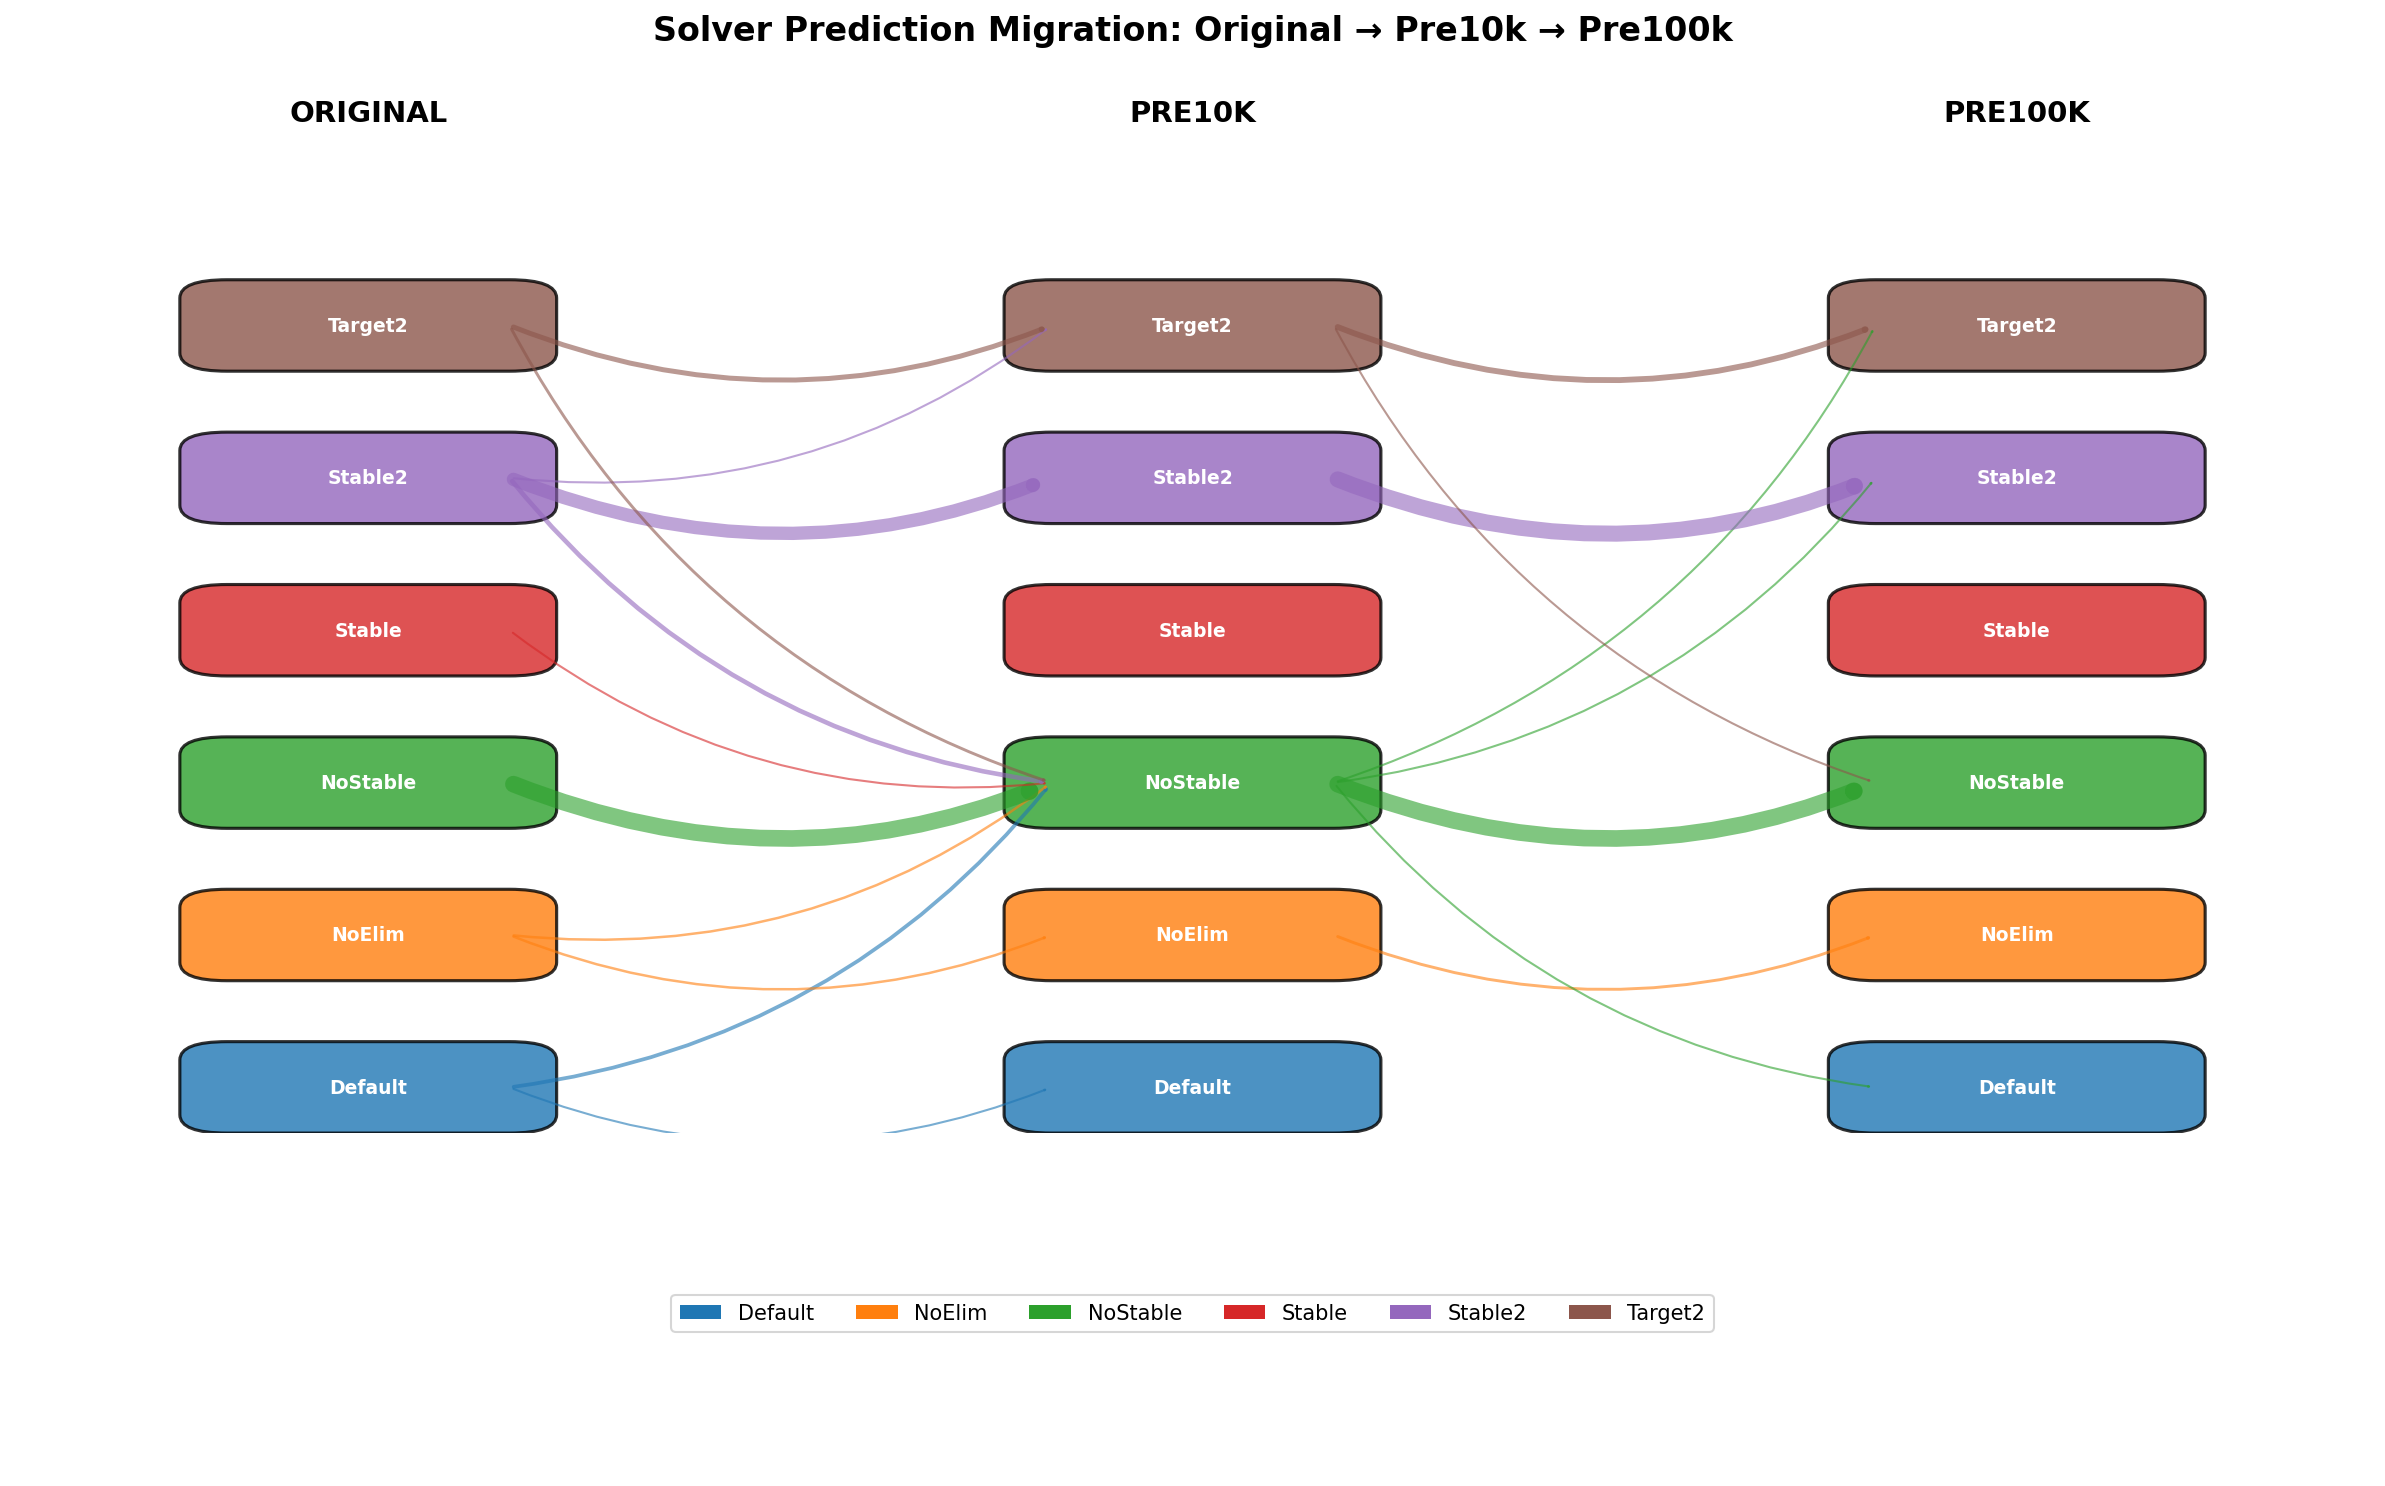
\includegraphics[width=0.9\textwidth]{assets/solver_migration_sankey.png}
    \caption{Änderung der jeweiligen Solver für Original-, Pre10k- und Pre100k-Benchmarks}
    \label{fig:solver_migration_sankey}
\end{figure}

Wichtigste Änderung: Der Großteil der Änderungen betrifft die Umstellung auf kissat\_nostable als empfohlenen Solver.

Die häufigsten Änderungen (Original $\rightarrow$ Pre10k):

\begin{table}[H]
    \centering
    \begin{tabular}{lccp{0.4\textwidth}}
        \toprule
        \textbf{Änderung} & \textbf{Anzahl} & \textbf{Bedeutung} \\
        \midrule
        stable2 $\rightarrow$ nostable & 28 & SATZilla wechselte von der Empfehlung stable2 zu nostable \\
        \midrule
        default $\rightarrow$ nostable & 15 & SATZilla wechselte von default zu nostable \\
        \midrule
        target2 $\rightarrow$ nostable & 12 & SATZilla wechselte von target2 zu nostable \\
        \bottomrule
    \end{tabular}
    \caption{Häufigste Änderungen (Original $\rightarrow$ Pre10k)}\label{tab:common_changes}
\end{table}

\newpage

\subsection{Abschließende Schlussfolgerung: Was uns diese Ergebnisse sagen}

Die drei in den Abschnitten 4.3.1 (Veränderungen der Vorhersageverteilung), 4.3.2 (Änderungen der Vorhersagen nach Vorverarbeitungsstufe) 
und 4.3.3 (Analyse der Solver-Migration) vorgestellten Analysen vermitteln insgesamt ein schlüssiges 
und aufschlussreiches Bild davon, wie sich die Vorverarbeitung auf die Solverauswahl von SATZilla auswirkt. 

\textbf{1. Die Vorverarbeitung verändert die Vorhersagensverteilung grundlegend}

Die Merkmale von SATZilla sind nicht vorverarbeitungsinvariant. Die von SATZilla berechneten Merkmale – wie 
beispielsweise das Verhältnis von Variablen zu Klauseln, Grapheigenschaften und Probing-Statistiken – 
ändern sich wesentlich, wenn eine Formel vereinfacht wird. Dies ist kein Fehler, sondern eine Folge 
der Tatsache, dass die Vorverarbeitung die Struktur der Formel tatsächlich verändert. Variablen 
werden eliminiert, Klauseln werden subsumiert, und die allgemeinen Verbindungsmuster des Graphen 
verschieben sich.

Das heißt aber nicht das die Vorhersagen der vereinfachten Benchmarks dann ünguldig sind, der neue 
empfohlende solver kann durchaus als der schnellste sein der dieses (vereinfachte) Problem lösen kann.

\textbf{2. Die Vorverarbeitung wirkt sich nicht auf alle Solver gleichermaßen aus}

Die „nostable“-Konfiguration – die die Heuristik der stabilen Phase deaktiviert – wird nach der 
Vorverarbeitung zum am häufigsten empfohlenen Löser. Ihr Anteil verdoppelt sich fast von 31,9 \% auf 
50,2 \%.

Dies liegt wahrscheinlich daran, dass kissat\_nostable sich besonders gut für vereinfachte Formeln 
eignet. Das Fehlen einer Heuristik für stabile Phasen kann von Vorteil sein, wenn die Formel bereits 
vereinfacht wurde.

\textbf{3. Die meisten Abweichungen treten während der anfänglichen Vereinfachung auf}

Dies deutet auf einen Effekt abnehmender Erträge hin: Die ersten 10.000 Vorverarbeitungsschritte 
bewirken die dramatischsten Veränderungen im Merkmalsraum. Weitere Vorverarbeitungsschritte 
(10.000 $\rightarrow$ 100.000) führen zu relativ geringeren zusätzlichen Veränderungen.

\textbf{4. Die Vorverarbeitung zeigt die Komplementarität der Solver}

Die Migrationsmuster zeigen, dass verschiedene Solver unterschiedliche "Komfortzonen" im Feature-Raum haben:
\begin{itemize}
    \item \textbf{nostable} gewinnt Instanzen von mehreren anderen Solvern (stable2, default, target2), was darauf hindeutet, dass vorverarbeitete Formeln gemeinsame Eigenschaften aufweisen, die nostable über ein breites Spektrum ursprünglicher Solver-Empfehlungen hinweg zur besten Wahl machen.
    \item \textbf{stable2} verliert Instanzen hauptsächlich an nostable, was darauf schließen lässt, dass die beiden Konfigurationen bei vorverarbeiteten Formeln austauschbar (Substitute) sind.
\end{itemize}

\textbf{5. Es besteht ein eindeutiger Zusammenhang zwischen Dosis und Wirkung}

Eine aggressivere Vorverarbeitung führt zu mehr Änderungen bei den Vorhersagen. Genau das würde ich 
erwarten, wenn die Merkmale von SATZilla aussagekräftige strukturelle Eigenschaften der Formeln erfassen.

Wären die SATZilla-Features oberflächlich oder vorverarbeitungsinvariant, würde man keinen Anstieg der Änderungsrate bei stärkerer Vorverarbeitung erwarten. Der beobachtete Anstieg (36,8\% $\rightarrow$ 41,5\%) bestätigt, dass:
\begin{itemize}
    \setlength{\itemsep}{0pt}
    \setlength{\parskip}{0pt}
    \setlength{\parsep}{0pt}
    \item Die Vorverarbeitung die Formelstruktur tatsächlich verändert
    \item Die SATZilla-Features diese Veränderungen erkennen
    \item Das Modell auf diese Feature-Änderungen mit aktualisierten Vorhersagen reagiert
\end{itemize}

Dies ist eine Validierung des SATZilla-Feature-Sets: Die Features sind sensitiv gegenüber echten 
strukturellen Veränderungen in der Formel.

\subsubsection{Fazit}

Die Analysen der Verschiebungen in der Vorhersageverteilung, der Änderungsraten über die verschiedenen 
Vorverarbeitungsstufen hinweg und der Solver-Migrationsmuster ergeben ein einheitliches Bild: Die 
Vorverarbeitung verändert die Solver-Empfehlungen von SATZilla grundlegend. Bei mehr als einem Drittel 
der Instanzen (36,8–41,5 \%) ändern sich die Vorhersagen, wobei eine aggressivere Vorverarbeitung 
zu mehr Änderungen führt.  

Die Migrationsanalyse zeigt, dass „nostable“ Instanzen von „stable2“, „default“ und „target2“ gewinnt, 
was darauf hindeutet, dass vorverarbeitete Formeln strukturelle Merkmale aufweisen, die diese 
Konfiguration begünstigen.

Die Dosis-Wirkungs-Beziehung – mehr Vorverarbeitung führt zu mehr Änderungen – bestätigt, dass die 
SATZilla-Merkmale empfindlich auf tatsächliche strukturelle Modifikationen in Formeln reagieren, 
was ihre Nützlichkeit für die Algorithmusauswahl bestätigt. 

Meiner Meinung nach sind die Vorhersagen von SATZilla auf vereinfachte Benchmarks immer noch von großer
relevanz, da die veränderten Vorhersagen durch die ebenfalls veränderten Eigenschaften entstanden sind 
und nicht weil SATZilla wahllos neue Empfehlungen macht.

Trotzdem sollte man in betracht ziehen, dass eine vereinfachung der Benchmarks immer zu verränderten Vorhersagen 
führen wird und ich hiermit in meiner Arbeit nicht bestätigen kann ob es auch dann immer der richtige (schnellste) 
Solver sein wird.

\newpage

\subsection{Vergleich der Featuresbedeutung für Pre10k und Pre100k}

Diese Analyse vergleicht die wichtigsten Features, die die Vorhersagen von SATZilla auf leicht vorverarbeiteten (Pre10k) gegenüber stark vorverarbeiteten (Pre100k) Benchmarks bestimmen. Durch das Training separater Random-Forest-Modelle auf jedem Datensatz und die Extraktion der Feature-Wichtigkeiten können wir verstehen:
\begin{itemize}
    \setlength{\itemsep}{0pt}
    \setlength{\parskip}{0pt}
    \setlength{\parsep}{0pt}
    \item Welche Features für die Solver-Auswahl bei vorverarbeiteten Formeln am wichtigsten sind
    \item Ob sich die Feature-Wichtigkeit mit der Intensität der Vorverarbeitung ändert
    \item Was dies darüber aussagt, wie die Vorverarbeitung die Formelstruktur beeinflusst
\end{itemize}

\subsubsection{Die Daten: Die 15 wichtigsten Merkmale für jede Vorverarbeitungsstufe}

\begin{figure}[H]
    \centering
    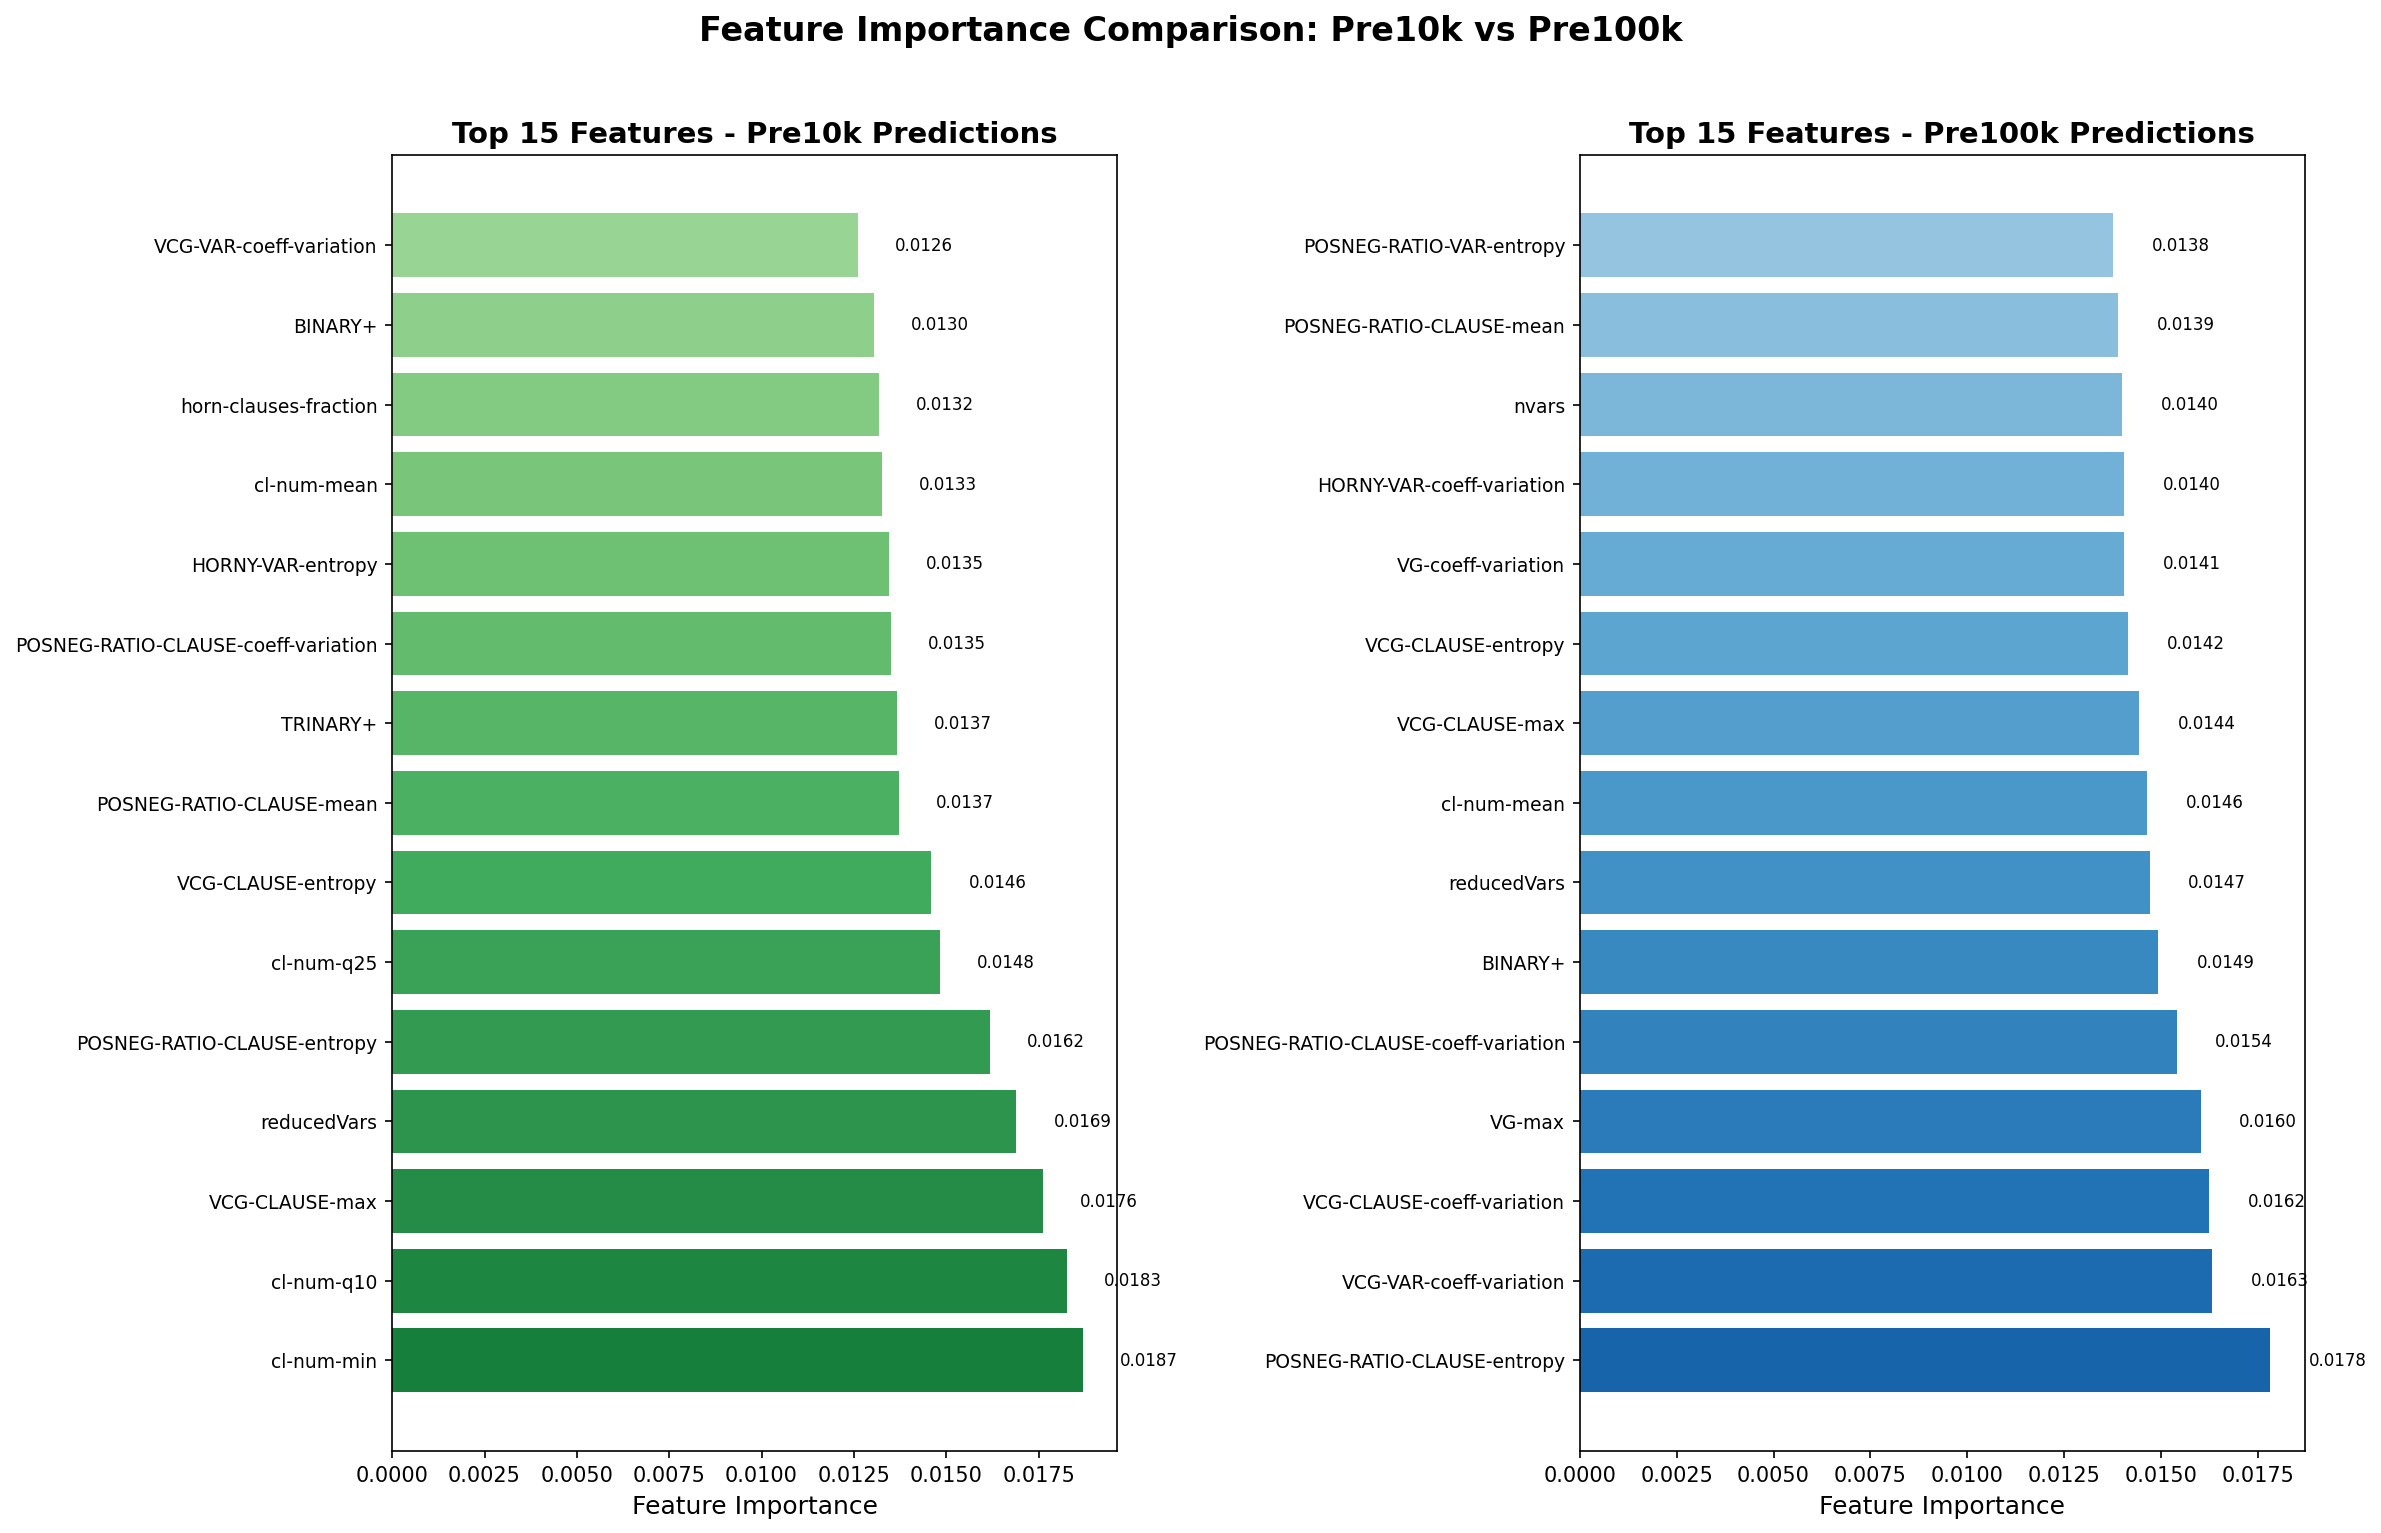
\includegraphics[width=0.95\textwidth]{assets/feature_importance_comparison.png}
    \caption{Vergleich der Top-15 Features von Pre10k- und Pre100k-Benchmarks}
    \label{fig:feature_importance_comparison}
\end{figure}

\textbf{Wichtigste Erkenntnise}

\textbf{1. Auf beiden Vorverarbeitungsstufen dominieren dieselben Features}

Die Top 10 der Merkmale sind bei Pre10k und Pre100k nahezu identisch, es gibt lediglich geringfügige 
Verschiebungen in der Rangfolge.

Die grundlegenden Faktoren für die Leistungsfähigkeit eines Solvers sind über alle Vorverarbeitungsstufen 
hinweg gleich. Selbst nach starker Vereinfachung entscheiden dieselben strukturellen Eigenschaften 
darüber, welcher Solver am schnellsten ist.

\textbf{2. Survey Propagation Features sind am wichtigsten}

SP-unconstraint-q50 (das 50. Perzentil der Wahrscheinlichkeiten für ungebundene Variablen aus der 
Survey-Propagation) ist das mit Abstand wichtigste Merkmal auf beiden Vorverarbeitungsstufen 
(Bedeutungswerte 0,0178 und 0,0185).

Die unconstraint Feature spiegelt die „Flexibilität“ der Formel wider. Formeln mit vielen unbeschränkten 
Variablen können von anderen Lösungsstrategien profitieren als stark eingeschränkte Formeln. Diese 
Eigenschaft bleibt auch nach der Vorverarbeitung erhalten.

\textbf{3. Graph-Based Features sind von großer Bedeutung}

In den Top 10 tauchen mehrere Features mit variable-clause graph (VCG) auf.

Variablen, die in vielen Klauseln vorkommen (hoher Grad), erzeugen Einschränkungen, die sich durch 
die gesamte Formel auswirken. Die Heuristiken des Solvers für die Variablenauswahl und die 
Neustartstrategien müssen sich an diese strukturellen Eigenschaften anpassen.

\textbf{4. Geringfügige Unterschiede zwischen Pre10k und Pre100k}

\begin{table}[H]
    \centering
    \begin{tabular}{lccc}
        \toprule
        \textbf{Feature} & \textbf{Pre10k Rang} & \textbf{Pre100k Rang} & \textbf{Änderung} \\
        \midrule
        reducedVars & 3 & 2 & Erhöhte Wichtigkeit \\
        \midrule
        SP-unconstraint-mean & 12 & 4 & Viel wichtiger \\
        \midrule
        SP-unconstraint-q90 & Nicht in Top 15 & 14 & Neu aufgenommen \\
        \midrule
        POSNEG-RATIO-VAR-stdev & 9 & 12 & Etwas weniger wichtig \\
        \bottomrule
    \end{tabular}
    \caption{Vergleich der Feature-Wichtigkeiten: Pre10k vs Pre100k}\label{tab:feature_importance_comparison}
\end{table}

Was uns diese unterschiede sagen:
\begin{itemize}
    \item „reducedVars“ gewinnt ab Pre100k an Bedeutung. Nach einer intensiven Vorverarbeitung ist die Anzahl der bei der Vereinfachung eliminierten Variablen ein aussagekräftigerer Indikator für die Leistung des Solvers. Das ist einleuchtend: Eine aggressivere Vorverarbeitung eliminiert mehr Variablen und verändert damit grundlegend die Größe und Struktur der Formel.
    \item Der SP-Mittelwert ohne Einschränkungen springt bei Pre100k von Rang 12 auf Rang 4. Die mittlere Wahrscheinlichkeit ohne Einschränkungen gewinnt nach einer intensiven Vorverarbeitung deutlich an Bedeutung. Dies deutet darauf hin, dass eine intensive Vorverarbeitung zu gleichmäßigeren Verteilungen der Variablen ohne Einschränkungen führt, wodurch der Mittelwert zu einer besseren zusammenfassenden Statistik wird als der Median.
    \item POSNEG-RATIO-VAR-stdev verliert bei Pre100k an Bedeutung. Die Variabilität der Verhältnisse zwischen positiven und negativen Literalen über die Variablen hinweg verliert nach einer umfassenden Vorverarbeitung an Aussagekraft, möglicherweise weil diese Verhältnisse durch die Vorverarbeitung ausgeglichen werden.
\end{itemize}

\subsection{Fazit}

Die Analyse der Featuressbedeutung zeigt, dass sowohl bei leicht als auch bei stark vorverarbeiteten 
Benchmarks dieselben strukturellen Eigenschaften die Auswahl des Solvers bestimmen. Merkmale der 
Survey-Propagation sind durchweg am wichtigsten, gefolgt von Merkmalen des Variablen-Klausel-Graphen 
und Statistiken zum Klausellernen. 

Während die Rangfolge der Merkmale weitgehend stabil bleibt, gewinnen reducedVars und SP-unconstraint-mean 
bei stärkerer Vorverarbeitung an Bedeutung, was widerspiegelt, wie eine aggressive Vereinfachung 
Variablen eliminiert und einheitlichere Verteilungen der unbeschränkten Variablen erzeugt. 

Diese Ergebnisse bestätigen die Robustheit des Merkmalsatzes von SATZilla über verschiedene 
Vorverarbeitungsstufen hinweg.

